\chapter{DISCUSSÃO DOS RESULTADOS} 

\par Neste capítulo são apresentados e discutidos os resultados obtidos por esta pesquisa e desenvolvimento do \textit{software}, apresentando os seus pontos positivos e negativos.

\par Inicialmente foram utilizadas as tecnologias Java, Primefaces e JSF, no entanto, viu-se a necessidade de alterar algumas destas tecnologias, visando a agilidade no processo de desenvolvimento. Desta forma, passou-se a utilizar HTML, CSS, Javascript em conjunto com o \textit{framework} Angular JS.

\par A mudança de tecnologias trouxe como benefício o desacoplamento das partes cliente (\textit{front-end}) e servidor (\textit{back end}), não sendo mais necessário recompilar, construir e publicar a aplicação no servidor \textit{web}, como era feito até então a cada alteração.

\par Após esta mudança, notou-se que a forma como o banco de dados era acessado deveria ser ajustada, a fim de seguir a mesma ideia proposta pela troca de tecnologias já mencionadas, uma vez que o banco de dados Neo4j permite duas maneiras de conexão, sendo elas: \textit{embedded} e por meio da API REST \cite{robinson_webber_eifrem_graph_databases}. Desta forma, passou-se a utilizar a API REST ao invés da forma \textit{embedded}, utilizada até então.

\par Com a mudança das tecnologias utilizadas no \textit{front end}, foi possível desenvolver uma aplicação com a interface \textit{clean} e moderna, permitindo ao usuário uma boa experiência de navegação. Também é possível citar, o uso do \textit{framework} Angular JS, que possibilitou não só o desenvolvimento ágil, como também a comunicação entre a aplicação e o \textit{web service}.

\par A linguagem Java, que foi utilizada para escrever todo o \textit{back end} deste trabalho, se mostrou uma ótima escolha, pois possui uma ampla biblioteca de materiais para apoio, disponibilizada pela Oracle, além de se integrar perfeitamente com o banco de dados Neo4j, que trás como exemplos, em sua documentação, aplicações que utilizam essas tecnologias em conjunto. Com a sua utilização obteve-se como resultado uma aplicação enquadrada nos padrões de desenvolvimento recomendados, além de ter um código legível e com qualidade, permitindo a utilização dos conceitos de orientação a objetos, o que facilitou o desenvolvimento da aplicação, pois permitiu o reaproveitamento de comportamentos por meio do conceito de herança e polimorfismo \cite{schildt_java_complete_reference}.

\par A fim de aplicar no desenvolvimento o mesmo conceito de relacionamentos, utilizado pela maioria das redes sociais, fez-se uso do banco de dados Neo4j em conjunto com a API \textit{Cypher}. Com o uso deste banco obteve-se como resultado uma aplicação cuja base de dados é toda orientada a grafos, deste modo, foi possível realizar consultas mais complexas de maneira simplificada, o que não seria possível com o uso de um banco de dados relacional, uma vez que para escrever este mesmo tipo de consulta seria necessário acessar várias tabelas por meio de \textit{joins}, deixando a consulta extensa e com baixa \textit{performance} \cite{sadalage_fowler_nosql_distilled_brief_guide}.

\par Neste escopo, concluiu-se o desenvolvimento desta aplicação, apresentando a seguir seus resultados mais relevantes.

\section{Localizar mão de obra}

\par Uma das funcionalidades implementadas no desenvolvimento foi a busca por mão de obra. Esta busca permite que o usuário encontre profissionais que desempenham a função específica procurada por ele. Para realizar esta busca, foi preciso escrever uma consulta que leva em conta três níveis de análise, sendo elas, a busca pelo profissional que desempenha o trabalho dentro da rede de parceiros do usuário, dentro da empresa onde o ele trabalha e por último, dentro da cidade onde vive.  

\par Para escrever esta consulta foi utilizada a tecnologia \textit{Cypher}, que é uma linguagem específica para o banco Neo4j \cite{neo4j_team_manual}. O Código~\ref{list:consulta_busca} apresenta a \textit{query} utilizada para realizar esta busca.

\par A Figura~\ref{fig:busca_domestica_edilson} demonstra a página apresentada ao usuário após realizar esta busca por um determinado serviço. No exemplo, é apresentado o resultado ao se realizar a busca por um profissional que desempenhe o serviço de doméstica.

\begin{figure}[h!]
	\centerline{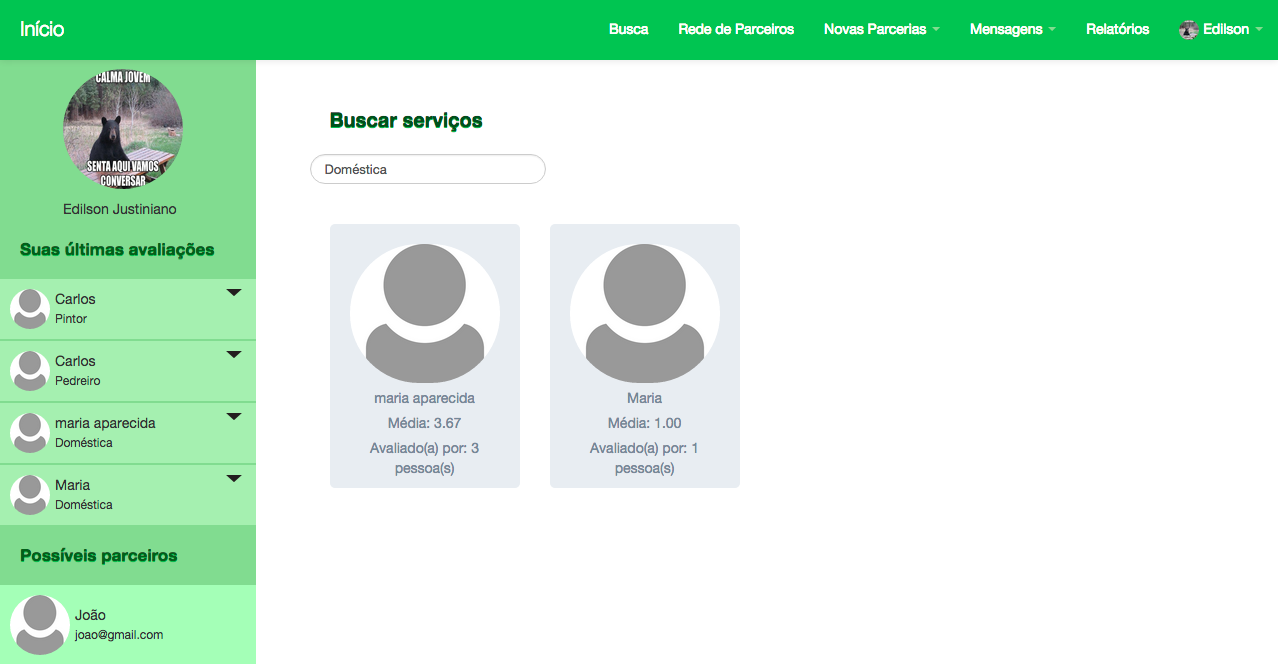
\includegraphics[scale=0.3]{./imagens/busca-domestica-edilson.png}}
	\caption[\textit Página resultante da busca por doméstica.]
	{\textit Página resultante da busca por doméstica \textbf{Fonte:} Elaborado pelos autores.}
	\label{fig:busca_domestica_edilson}
\end{figure}

\par A ideia desta funcionalidade foi apresentar um possível prestador de serviços que já tenha sido avaliado por alguém em comum ao usuário solicitante, desta forma, há uma confiança maior em relação ao profissional que está sendo contratado. Portanto, essa busca irá apresentar diferentes prestadores de serviços, incluindo as médias de cada um deles, a cada usuário solicitante.

\par O uso de um banco de dados orientado a grafos como o Neo4j simplificou a forma de obter este resultado, uma vez que ao utilizar um banco relacional, o mesmo resultado poderia ser obtido, porém o gasto em processamento  e \textit{performance} seria extremamente maior. A API \textit{Cypher} facilitou a escrita de todas as consultas inclusive essa, por meio dela foi possível desenvolver consultas mais complexas como esta de forma mais rápida, agilizando o desenvolvimento da principal parte do trabalho.





\section{Apresentar possíveis parceiros}

\par Esta funcionalidade apresenta ao usuário possíveis parceiros que poderão compor a sua rede de relacionamentos. Para realizar esta busca, também foi preciso escrever uma consulta que levasse em conta dois níveis de análise, sendo elas, a busca pelo possível parceiro dentro da empresa onde o usuário trabalha, levando em conta a quantidade de parceiros em comum entre ambos (usuário autenticado e o possível parceiro) e a busca por parceiros dentro da mesma cidade, também seguindo este mesmo critério. O Código~\ref{list:consulta_possiveis_parceiros} apresenta a \textit{query} utilizada para realizar esta busca.

\par A Figura~\ref{fig:busca_possiveis_parceiros} apresenta o resultado da busca por possíveis parceiros, contendo uma lista com as pessoas que atendam os requisitos pré estabelecidos na consulta.

\begin{figure}[h!]
	\centerline{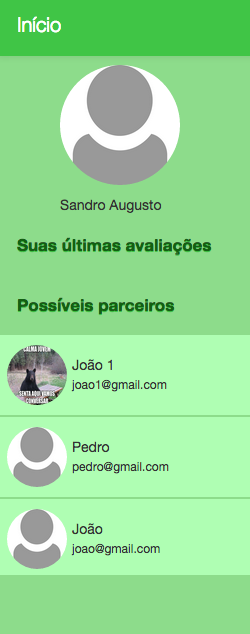
\includegraphics[scale=0.4]{./imagens/busca-possiveis-parceiros.png}}
	\caption[Funcionalidade que apresenta a lista com possíveis parceiros]
	{Funcionalidade que apresenta a lista com possíveis parceiros \textbf{Fonte:} Elaborado pelos autores.}
	\label{fig:busca_possiveis_parceiros}
\end{figure}

\par A ideia desta funcionalidade foi apresentar um possível parceiro que provavelmente já tenha algum vínculo com o usuário ou que possua afinidade com alguém da sua rede de parceria.

\section{Localizar novos parceiros}

\par Esta busca permite ao usuário encontrar novos parceiros para compor a sua rede de relacionamentos. Para realizar esta busca, utilizou-se uma consulta muito semelhante a da funcionalidade anterior, acrescentando apenas o filtro para permitir a busca por nomes informado pelo usuário.

\par Para auxiliar o usuário nessa tarefa, foi criada uma nova consulta que leva em consideração apenas o nome do usuário, visando a sua localização independente de relacionamentos. Essa consulta é realizada apenas quando o número de resultados encontrados pelo nome informado pelo usuário for menor que um determinado valor definido, nesse caso, cinco.

\par A Figura~\ref{fig:busca_novos_parceiros} apresenta o resultado da busca por novos parceiros, contendo uma lista com as pessoas que atendam os requisitos pré estabelecidos na consulta.

\begin{figure}[h!]
	\centerline{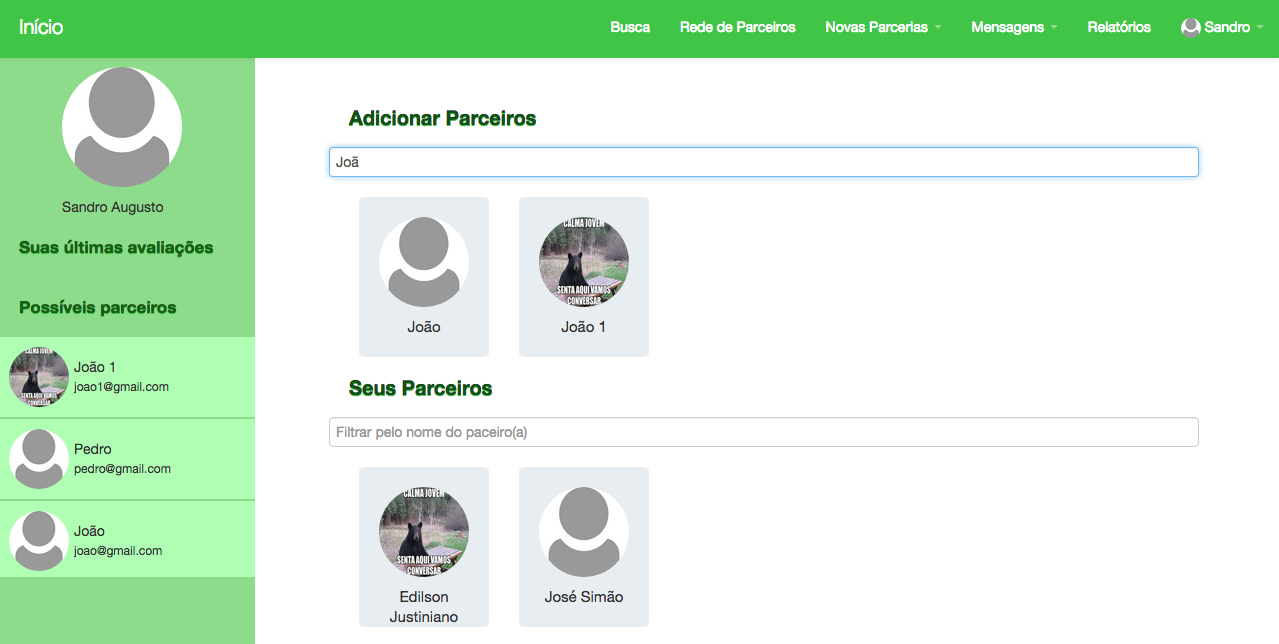
\includegraphics[scale=0.3]{./imagens/busca-novos-parceiros.png}}
	\caption[Funcionalidade que apresenta a busca por novos parceiros]
	{Funcionalidade que apresenta a busca por novos parceiros. \textbf{Fonte:} Elaborado pelos autores.}
	\label{fig:busca_novos_parceiros}
\end{figure}

\par  Esta funcionalidade permite então que o usuário localize novos parceiros, que são indicados por ele e não sugeridos pelo sistema, como acontece na funcionalidade anterior.

\par Neste capítulo foram apresentados os resultados mais relevantes obtidos por esta pesquisa, sendo eles satisfatórios, pois atenderam aos objetivos propostos por este trabalho.